% Compile from this folder, keeping initial_pic/ and fig/ alongside this file.
\documentclass[25pt,a0paper,portrait,margin=1.8cm,
  innermargin=0pt,blockverticalspace=1.5cm,colspace=1.6cm]{tikzposter}
\geometry{paperwidth=60cm,paperheight=120cm}
\makeatletter
\setlength{\TP@visibletextwidth}{\textwidth-2\TP@innermargin}
\setlength{\TP@visibletextheight}{\textheight-2\TP@innermargin}
\makeatother

\usepackage[T1]{fontenc}
\usepackage{lmodern}
\usepackage{graphicx}
\usepackage{enumitem}
\usepackage{amsmath,amssymb}
\renewcommand{\familydefault}{\rmdefault}
\graphicspath{{initial_pic/}{fig/}}
\tikzposterlatexaffectionproofoff

\definecolor{tdliblue}{RGB}{0,64,152}
\definecolor{bandblue}{RGB}{16,47,90}
\colorlet{backgroundcolor}{white}
\colorlet{titlebgcolor}{white}
\colorlet{titlefgcolor}{black}
\colorlet{blocktitlebgcolor}{white}
\colorlet{blocktitlefgcolor}{tdliblue}
\colorlet{blockbodybgcolor}{white}
\colorlet{blockbodyfgcolor}{black}
\setlist[itemize]{leftmargin=1.1cm,itemsep=0.35cm,topsep=0.3cm}
\usebackgroundstyle{Empty}
% Paint the bands at page level so they reach past tikzposter's margin clip.
\AddToHook{shipout/background}{%
  \begin{tikzpicture}[remember picture,overlay]
    \fill[bandblue] (current page.north west) rectangle
      ([yshift=-14.6cm]current page.north east);
    \fill[bandblue] (current page.south west) rectangle
      ([yshift=7.2cm]current page.south east);
  \end{tikzpicture}%
}

% Replace the title and author names; the affiliation is already set.
\newcommand{\postertitle}{Your poster title goes here\\An optional second line}
\title{\postertitle}
\author{First Author$^1$, Second Author$^1$, Third Author$^1$}
\institute{$^1$Tsung-Dao Lee Institute, Shanghai Jiao Tong University}

\definetitlestyle{Minimal}{
  width=56.4cm,roundedcorners=12,linewidth=1pt,innersep=0.6cm,
  titletotopverticalspace=0cm,titletoblockverticalspace=1.4cm
}{
  \draw[draw=gray!30,fill=white,line width=\titlelinewidth,
    rounded corners=\titleroundedcorners]
    (\titleposleft,\titleposbottom) rectangle (\titleposright,\titlepostop);
}
\usetitlestyle{Minimal}

\makeatletter
% Correct tikzposter 2.0's assignment of its title-scale macro.
\define@key{title}{titletextscale}{\def\TP@titletextscale{#1}}
\renewcommand{\TP@maketitle}{%
  \begin{minipage}[c]{8cm}
    
\includegraphics[width=8cm]{sjtu1.png}
  \end{minipage}\hspace{1.1cm}%
  \begin{minipage}[c]{45cm}
    {\fontsize{76}{86}\selectfont\bfseries\postertitle\par}
    \vspace{0.7cm}
    \begin{minipage}[c]{35cm}
      {\fontsize{35}{43}\selectfont\@author\par}
      \vspace{0.3cm}
      {\fontsize{28}{35}\selectfont\@institute\par}
    \end{minipage}\hfill
    \begin{minipage}[c]{8.5cm}
      
\includegraphics[width=8.5cm]{LHAASO1.png}
    \end{minipage}
  \end{minipage}%
}
\makeatother

\defineblockstyle{Minimal}{
  titlewidthscale=1,bodywidthscale=1,titleleft,
  titleoffsetx=0pt,titleoffsety=0pt,bodyoffsetx=0pt,bodyoffsety=0pt,
  bodyverticalshift=0pt,roundedcorners=0,linewidth=1pt,
  titleinnersep=0.6cm,bodyinnersep=0.6cm
}{
  \draw[draw=tdliblue!30,line width=1pt]
    (blocktitle.south west) -- (blocktitle.south east);
}
\useblockstyle{Minimal}

% Replace each empty figure box with \includegraphics[width=\linewidth]{...}.
\newcommand{\figureplaceholder}[1]{%
  \par\noindent\fcolorbox{gray!30}{white}{%
    \parbox[c][#1][c]{\dimexpr\linewidth-2\fboxsep-2\fboxrule\relax}{%
      \centering\color{gray}\fontsize{28}{36}\selectfont Figure}}
  \par
}

\begin{document}
\maketitle
\fontsize{30}{39}\selectfont

\begin{columns}
  \column{0.5}
  \block{1. Introduction}{
    Background and motivation.
    \begin{itemize}
      \item Scientific context.
      \item Research question.
    \end{itemize}
    \vspace{4cm}
  }

  \block{2. Methods}{
    \begin{itemize}
      \item Data sample and observation period.
      \item Selection criteria.
      \item Analysis method.
    \end{itemize}
    \vspace{0.8cm}
    \figureplaceholder{30cm}
    {\fontsize{26}{33}\selectfont Figure 1. Caption.\par}
    \vspace{1.8cm}
    Analysis details.
    \vspace{1.2cm}
    \figureplaceholder{30cm}
    {\fontsize{26}{33}\selectfont Figure 2. Caption.\par}
  }

  \column{0.5}
  \block{3. Conclusion}{
    \begin{itemize}
      \item Main result.
      \item Interpretation.
    \end{itemize}
    \vspace{0.8cm}
    \figureplaceholder{33cm}
    {\fontsize{26}{33}\selectfont Figure 3. Caption.\par}
    \vspace{1.8cm}
    \figureplaceholder{33cm}
    {\fontsize{26}{33}\selectfont Figure 4. Caption.\par}
  }

  \block{Summary}{
    \begin{itemize}
      \item Main finding.
      \item Implication.
    \end{itemize}
  }
\end{columns}

% Page-level placement keeps the footer clear of tikzposter's margin clip.
\AddToHook{shipout/foreground}{%
\begin{tikzpicture}[remember picture,overlay]
% Crop the seal and empty edges from the 300 dpi original; keep both name lines.
\node[anchor=center,inner sep=0pt]
  at ([yshift=4.9cm]current page.south)
  {
\includegraphics[trim=122.64bp 6.24bp 0.24bp 6.48bp,clip,width=9cm]{tdli-logo-white.png}};
\node[anchor=center,inner sep=0pt,text=white]
  at ([yshift=1.45cm]current page.south)
  {\fontsize{26}{33}\selectfont Contact: your.name@sjtu.edu.cn};
% Preserve the reference poster's transparent white TDLI building drawing.
\node[anchor=west,inner sep=0pt]
  at ([xshift=2.4cm,yshift=3.6cm]current page.south west)
  {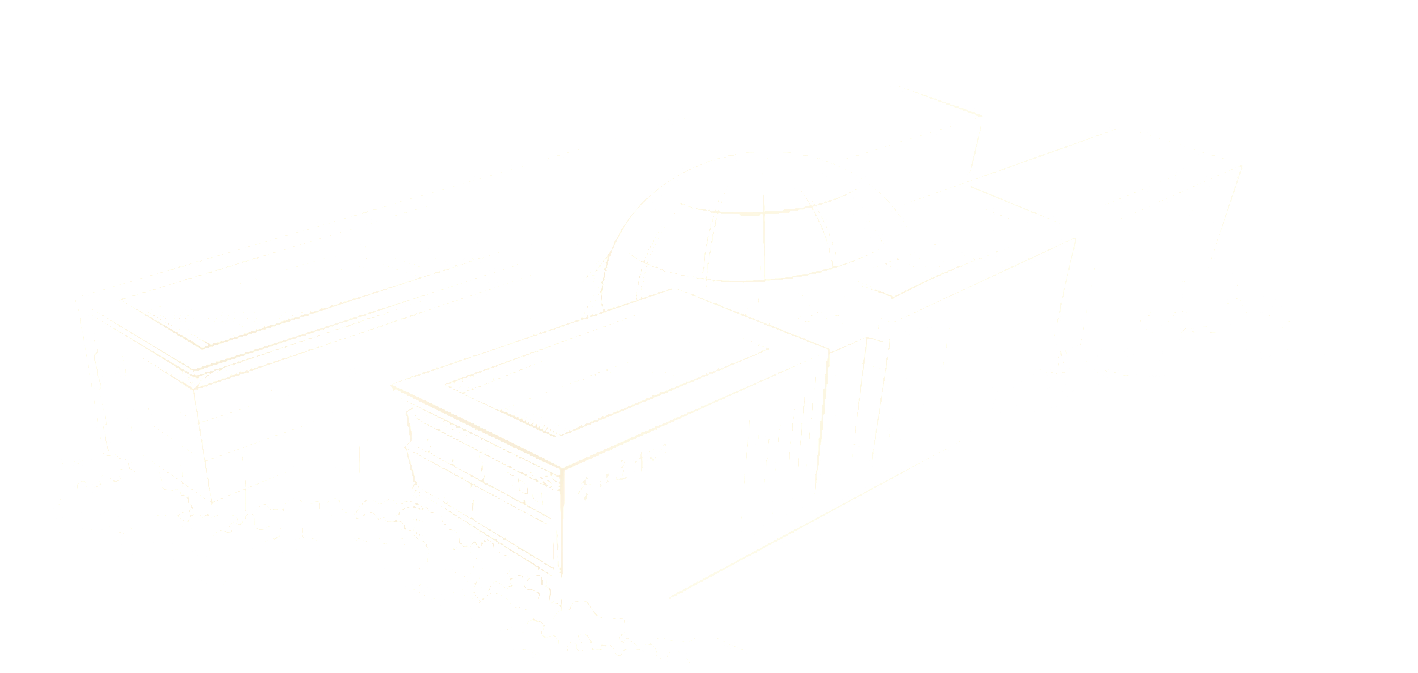
\includegraphics[width=11.2cm]{tdlibg.png}};
% Replace this square with your own QR image, not the reference author's code.
\node[anchor=east,inner sep=0pt]
  at ([xshift=-2.4cm,yshift=3.6cm]current page.south east)
  {\fcolorbox{gray!30}{white}{%
    \parbox[c][4.8cm][c]{4.8cm}{%
      \centering\color{gray}\fontsize{26}{33}\selectfont QR code}}};
\end{tikzpicture}%
}
\end{document}
